\section{Worked example}\label{sec:example}

We fit one public cohort end to end: the control females of the genetically heterogeneous UM-HET3 mice of the NIA
Interventions Testing Program \citep{nadon2008design}, cohort C2016, three sites pooled
(Mouse Phenome Database, project ITP1; the pooling rule was fixed before the fit).
% src: ~/code/sraging/examples/data/SOURCE.md (data source, terms of use and sha256; MPD waiver of copyright with citation requirement)
The input is a two-column table of death or removal age in days and an event indicator (1 = death, 0 = censored):
\C{ex-n} individuals, \C{ex-deaths} deaths and \C{ex-n-cens} individual removed alive at day \C{ex-km-day}
(Figure~\ref{fig:example}). Deaths are recorded to the day, so $\delta=1$. The fit is one command,
\begin{verbatim}
sraging fit-cohort --csv itp_c2016_het3_control_female.csv --delta 1
\end{verbatim}
which runs the default calibrator, \code{profile_jax2} 1.0.1, with the two combination claims and the leverage check
(the numbers below are those of the run stored with the package's examples). For this paper we reran the command
with the package code of tag \code{v0.1.0}, which the released tag \code{v0.1.1} keeps unchanged: none of the \C{ex-refit-ncomp} numbers compared (the estimates, the
log-likelihood, every claim's shape and ends, the two combination claims and the leverage verdict) changed in any digit,
and the rerun also records the ends of $\kappa$'s range (below).
% src: tables/example_refit_v010.json (the refit), tables/example_refit_check.{py,csv} (the comparison)
Figure~\ref{fig:example} overlays the model on the data: the fitted survival curve follows the Kaplan--Meier curve over the whole lifespan, and the model hazard follows
the data's hazard over three orders of magnitude, except for the \C{ex-deaths-first-year} deaths of the first year, which
are more frequent than the model predicts.

\begin{figure}[t]
  \centering
  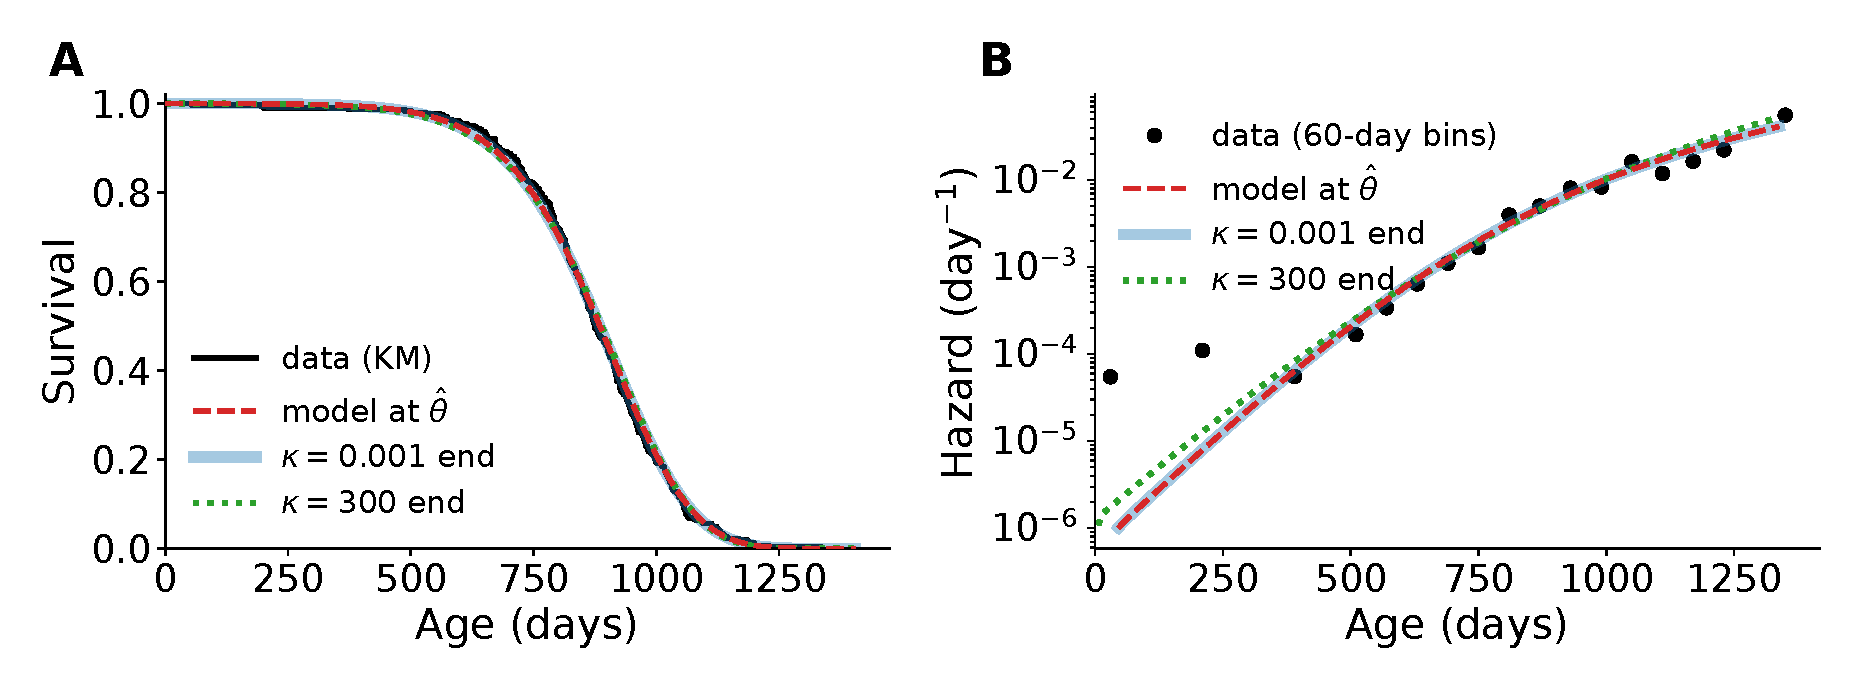
\includegraphics[width=\linewidth]{fig_example.pdf}
  \caption{\textbf{Data and fitted model of the worked example} (UM-HET3 control females, cohort C2016,
  $n=\C{ex-n}$). \textbf{A}, Kaplan--Meier survival of the data (solid) and the model's survival curve at the stored
  maximum-likelihood estimate $\hat\theta$ (dashed), computed by one evaluation of the engine, and at the two ends of
  $\kappa$'s range recorded by the refit: points within 1.92 nats of the best fit at $\kappa=\C{ex-kend-lo}$ (wide pale
  line, under $\hat\theta$) and $\kappa=\C{ex-kend-hi}$ (dotted), the two edges of the prior box. \textbf{B}, the data's
  hazard in 60-day bins (deaths divided by days at risk) and the model hazard at the same three points. The two leftmost
  points hold the \C{ex-deaths-first-year} deaths of the first year.}
  \label{fig:example}
\end{figure}

\begin{table}[t]
  \centering\small
  \caption{\textbf{Claims of the worked example} (95\,\% profile-likelihood intervals, stored fit, time unit days).
  The upper ends of $\eta$, $\beta$ and $\eta/\eps$ are set by the prior box ($\kappa\le300$), not by the data.}
  \label{tab:example}
  \begin{tabular}{@{}lllll@{}}
    \toprule
    Quantity & Claim shape & Point & 95\,\% interval & Read as \\
    \midrule
    $\eta$ (day$^{-2}$) & value & \C{ex-t-eta-pt} & [\C{ex-t-eta-lo}, \C{ex-t-eta-hi}] & value; lower end from the data \\
    $\eps$ (day$^{-1}$) & value & \C{ex-t-eps-pt} & [\C{ex-t-eps-lo}, \C{ex-t-eps-hi}] & value \\
    $\beta$ (day$^{-1}$) & bound & not reported & $\ge$ \C{ex-t-beta-lo} (upper end \C{ex-t-beta-hi}: box) & lower bound only \\
    $\kappa$ & no claim & not reported & --- & not determined \\
    $\eta/\eps$ (day$^{-1}$) & value & \C{ex-t-ratio-pt} & [\C{ex-t-ratio-lo}, \C{ex-t-ratio-hi}] & value \\
    $\beta\rbar/\eta$ (days) & value & \C{ex-t-rbar-pt} & [\C{ex-t-rbar-lo}, \C{ex-t-rbar-hi}] & value \\
    \bottomrule
  \end{tabular}
\end{table}

\paragraph{Reading the output.} $\eta$ and $\eps$ are values with finite intervals, about an order of magnitude wide.
The point estimates of $\kappa$ and $\beta$ are not reported as estimates: the profile of $\kappa$ is flat over the
whole prior box, so the fit prints a representative $\kappa$ and no claim, and $\beta$ moves along a ridge with $\kappa$.
The fit records how far the ridge reaches (the key \code{kappa\_ends} of its diagnostics, which \code{sraging}'s
overlay plot draws): points within 1.92 nats of the best fit lie at both edges of the box, $\kappa=\C{ex-kend-lo}$ and
$\kappa=\C{ex-kend-hi}$. From one end to the other $\beta$ grows about \C{ex-kend-beta-fold}-fold and $\eta$ and $\eps$
grow \C{ex-kend-eta-fold}- and \C{ex-kend-eps-fold}-fold, while $\eta/\eps$ moves only from \C{ex-kend-ratio-lo} to
\C{ex-kend-ratio-hi}, inside its interval. The model curves at the two ends differ in survival by at most \C{ex-kend-dS},
and their hazards are within a factor \C{ex-kend-hz-mid} of each other from day \C{ex-kend-mid-from} on, the ages of the
central 98\,\% of the model's deaths (Figure~\ref{fig:example}); before that, where the hazard is about $10^{-4}$ per day
or less, they differ by up to a factor \C{ex-kend-hz-max}.
% src: tables/example_kappa_ends.{py,csv}, tables/example_kappa_ends_summary.csv
The data constrain $\beta$ only through its lower end and through the mean removal $\beta\rbar(\kappa)$: the
combination $\beta\rbar/\eta$ is a value, \C{ex-t-rbar-pt} days (\C{ex-t-rbar-lo}--\C{ex-t-rbar-hi}), which against the
cohort's lifespan scale $L=\C{ex-L}$ days is a ballistic score $B=\beta\rbar/(\eta L)$ of \C{ex-B-pt}
(\C{ex-B-lo}--\C{ex-B-hi}). $\eta/\eps$ is also a value. The coverage of the two combination claims was measured for version 1.0.1 on the
previous benchmark library only (Table~\ref{tab:identified}, note c; Section~\ref{sec:limitations}).

\paragraph{Leverage.} The check removes the individual with the largest one-step influence (a death at day
\C{ex-lev-age}) and refits. The four quantities $\eta$, $\eps$, $\eta/\eps$ and $\beta\rbar/\eta$ move by up to a factor
\C{ex-lev-R4}, but the refit gains only \C{ex-lev-gain} nats, below the \C{ex-lev-nats} nats of the flag rule
(factor \C{ex-lev-ratio} and \C{ex-lev-nats} nats together are required), so the verdict is a flat-valley slide, not a
flag; the two combination claims move by at most \C{ex-lev-Rlead}. No warning fired.

\paragraph{Cost.} In the stored run the fit took \C{ex-cpu} CPU-s (in the rerun \C{ex-refit-cpu}, on the same laptop); the combination claims cost \C{ex-comb-ratio} times that and the
leverage check \C{ex-lev-share}\,\% of it, for a total wall time of \C{ex-wall-s}\,s on one laptop process.
